\section{System overview}
The system basically consists out of two parts: a user interface front-end and
a database backend. The user-interface contains a tool to generate graphical
expressions who are compiled to an intermediate code based on XML (we could
compare this with for instance Java bytecode). The database backend can read
this code and executes it. Furthermore it can answer the queries by sending
back results formatted by XML. In this way we can look at the front-end as a
compiler and the backend as a runtime environment. It is important to note that
the user-interface only checks for language consistency. For instance it checks
if the primitives are ordered appropriately, but doesn't check for instance if
a certain country actually exists in the database. The backend assumes the
entered intermediate code is consistent and only executes the queries. Both
parts are written in \Csh{}. The database part invokes a \texttt{PostgreSQL}
database.
\paragraph{}
Figure \ref{fig:systemOverview} gives a graphical overview of the system.
\begin{figure}[hbt]
\centering
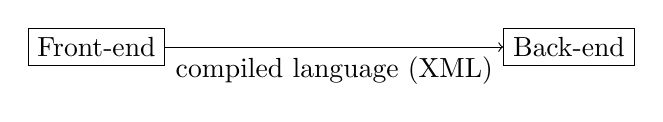
\begin{tikzpicture}
\node[rectangle,draw=black] (F) at (-3,0) {Front-end};
\node[rectangle,draw=black] (B) at (3,0) {Back-end};
\draw[->] (F) to node[below]{compiled language (XML)} (B);
\end{tikzpicture}
\caption{Graphical overview of the System}
\label{fig:systemOverview}
\end{figure}
\paragraph{}We will describe each of the parts in detail in the sections below.